\documentclass[final]{beamer} % beamer 3.10: do NOT use option hyperref={pdfpagelabels=false} !
  %\documentclass[final,hyperref={pdfpagelabels=false}]{beamer} % beamer 3.07: get rid of beamer warnings
\mode<presentation> {  %% check http://www-i6.informatik.rwth-aachen.de/~dreuw/latexbeamerposter.php for examples
	\usetheme{JK}    %% you should define your own theme e.g. for big headlines using your own logos 
}

\setbeamertemplate{caption}[numbered] 
\usepackage[english]{babel}
\usepackage{framed}
\usepackage[utf8]{inputenc}
\usepackage{amsmath,amsthm, amssymb, latexsym}
\usepackage{booktabs} % nice tables
\usepackage{multirow}
\usepackage{sidecap}
\usepackage{soul}
\usepackage{setspace}

\newcommand{\mr}[2]{\multirow{#1}{*}{#2}}  
\newcommand{\mc}[3]{\multicolumn{#1}{#2}{#3}}  

\newcommand{\tcb}[1]{\textcolor{blue}{#1}}
\newcommand{\tcr}[1]{\textcolor{red}{#1}}

%\usepackage{times}\usefonttheme{professionalfonts}  % times is obsolete
%  \usepackage[absolute,overlay]{textpos}
\usefonttheme[onlymath]{serif}
\boldmath
\usepackage[orientation=portrait,size=a0,scale=1.4,debug]{beamerposter}                       % e.g. for DIN-A0 poster
%\usepackage[orientation=portrait,size=a1,scale=1.4,grid,debug]{beamerposter}                  % e.g. for DIN-A1 poster, with optional grid and debug output
%\usepackage[size=custom,width=200,height=120,scale=2,debug]{beamerposter}                     % e.g. for custom size poster
%\usepackage[orientation=portrait,size=a0,scale=1.0,printer=rwth-glossy-uv.df]{beamerposter}   % e.g. for DIN-A0 poster with rwth-glossy-uv printer check
% ...
%
\title{Analytical and Monte-Carlo modeling of Multi-Parallel Slit and Knife-Edge Slit Prompt Gamma Cameras}
\author{E. Testa\inst{1}, B.F.B. Huisman\inst{1,2}, D. Dauvergne\inst{3}, J. M. L\'etang\inst{2}, D. Sarrut\inst{3}}
\institute[]{
	\inst{1} Universit{\'e} de Lyon, Universit{\'e} Claude Bernard Lyon 1, CNRS/IN2P3, Institut de Physique Nucl{\'e}aire de Lyon, 69622 Villeurbanne, France, \inst{2} CREATIS, Université de Lyon; CNRS UMR5220; INSERM U1044; INSA-Lyon; Université Lyon 1; Centre Léon Bérard, Lyon, France, \inst{3} Universit\'e Grenoble Alpes, Laboratoire de Physique Subatomique et de Cosmologie, CNRS/IN2P3, Grenoble, France}
\footer{contact: e.testa@ipnl.in2p3.fr}

\begin{document}
	
\begin{frame}{} 
\vfill
  
%%%%%%%%%%%%%%%%%%%%%%%%%%%%%%%%%%%%%%%%%%%%%%%%%%%%%%%%%%%%%%%%%%%%%%%%    
\begin{block}{Introduction}
	\begin{columns}[t]
		\begin{column}{0.49\textwidth}
			\centering{\Red{\large{Ion-range verification during hadrontherapy}}}
			\begin{itemize}
				\item Major challenge to fully take benefit from ion beam ballistic properties
				\item Main imaging modalities under study:  prompt gammas (PG) detection \cite{Krimmer2017a} with non-imaging systems (such as PG Timing, PG Spectroscopy and PG Peak Integral) and imaging systems, namely physically-collimated or electronically collimated cameras (Compton cameras)
			\end{itemize}
		
		\end{column}

		\begin{column}{0.49\textwidth}
			\centering{\Red{\large{PG collimated cameras}}}
			\begin{itemize}
				\item 2 main collimator configurations: Multi-Parallel Slit (MPS) \cite{Pinto2014} and Knife-Edge Slit (KES) collimators \cite{Smeets2012} (Figure XXX)
				\item No theoretical considerations have been proposed for the specific 1D collimation systems developed for PG detection 
			\end{itemize}			
		\end{column}
	\end{columns}

\end{block} % introduction
%%%%%%%%%%%%%%%%%%%%%%%%%%%%%%%%%%%%%%%%%%%%%%%%%%%%%%%%%%%%%%%%%%%%%%%%

\begin{columns}[t]
	
	\begin{column}{0.49\textwidth}
	  \vspace{-2ex}
	  %%%%%%%%%%%%%%%%%%%%%%%%%%%%%%%%%%%%%%%%%%%%%%%%%%%%%%
	  \begin{block}{Objectives}
			\begin{itemize}
				\item Development an analytical model (AM) of MPS and KES collimations $\Rightarrow$ main intrinsic features of each collimator
				\item Verification of the AM by means of Monte Carlo (MC) simulations 
				\item Comparison the two MPS and KES prototypes developed by IBA and the CLaRyS collaboration, respectively.
			\end{itemize}				    
	  \end{block}
		
	  %%%%%%%%%%%%%%%%%%%%%%%%%%%%%%%%%%%%%%%%%%%%%%%%%%%%%%
	  \begin{block}{The Analytical Model of MPS and KES collimations}
			
% 			\begin{columns}[t]
% 				\begin{column}{0.7\textwidth}
					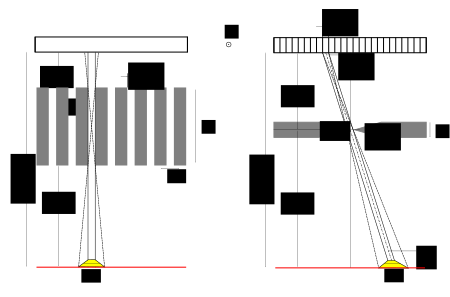
\includegraphics[width=0.7\textwidth]{./figures/MPS-KES_scheme}
% 				\end{column}

% 				\begin{column}{0.3\textwidth}
					
					\begin{table}[h]
					\small
					\centering
					\begin{tabular}{lcc}
						\midrule
																				& MPS                              & KES \\
						\midrule
						Effective slit width ($s_e$)& $s$                              & $s + \frac{\ln(2)}{\mu~\tan(\alpha)}$ \\
						Spatial resolution (Res)		& $s \left(1+\frac{d_1}{D}\right)$ & $s_e \left( 1+\frac{d_1^{'}}{d_2^{'}} \right)$ \\
						Detection efficiency (Eff)	& $\frac{H s}{ 4 \pi L D } (1-f) $ & $\frac{H s_e}{ 4 \pi L d_2^{'} } \left( 1 + \frac{x^2}{d_2^{'2}} \right)^{-3/2} $ \\
						Collimator effective thickness ($T_e$) & $D\times f$           & $T$ \\
						\midrule
					\end{tabular}
					\caption{Detection efficiencies and spatial resolution predicted by the analytical model}
					\end{table}
					
% 				\end{column}
% 			\end{columns}
	  \end{block}
	  %%%%%%%%%%%%%%%%%%%%%%%%%%%%%%%%%%%%%%%%%%%%%%%%%%%%%%
		
	  \begin{block}{Monte Carlo simulations}
			
			\begin{itemize}
				\item Gate 7.2 with Geant4 4.10.02 and the QGSP\_BIC\_HP\_EMY physics list
				\item Optimization: vpgTLE variance reduction method $\Rightarrow$ gain of $\sim 10^3$ \cite{Huisman2016}
				\item Background (BKG) modeling: 
				\begin{itemize}
					\item Estimates of background counts in the detector are taken from \cite{Perali2014} (KES, $2.5\cdot10^{-7}$ counts/incident proton and per 8~mm bin) and \cite{Pinto2014} (MPS, $5 \cdot 10^{-7}$ counts per primary proton per 4~mm bin) which are both based on measured data

				\end{itemize}

			\end{itemize}

	  \end{block}		
		
	  \begin{block}{Figures of merit}
			
			\begin{itemize}
				\item Detection efficiency: \#detected PG/\#emitted PG in the camera Field of View (FOV)
				\item Spatial resolution: the width of the PG profile fall-off, namely the FWHM of the peak resulting from the computation of the PG profile first derivative
				\item Fall-off Retrieval Precision (FRP): \tcr{TODO}
			\end{itemize}


	  \end{block}				
		
			  %%%%%%%%%%%%%%%%%%%%%%%%%%%%%%%%%%%%%%%%%%%%%%%%%%%%%% 
	  \begin{block}{References}
	    \tiny
% 			\begin{spacing}{0.5}
	    \setbeamertemplate{bibliography item}[text] 
%	    \bibliographystyle{elsarticle-num}
	    \bibliographystyle{ieeetr}
	    \bibliography{biblio_abb}				
% 			\end{spacing}


	  \end{block}
       
	  %%%%%%%%%%%%%%%%%%%%%%%%%%%%%%%%%%%%%%%%%%%%%%%%%%%%%%    
	\end{column} % end of left column
	
	\begin{column}{0.49\textwidth} % right column
	  \vspace{-2ex}
		%%%%%%%%%%%%%%%%%%%%%%%%%%%%%%%%%%%%%%%%%%%%%%%%%%%%%%  
		\begin{block}{Simulated geometries}
		
					\begin{itemize}
						\item 2 configurations (Table~\ref{CamerasParameters}):
						\begin{itemize}
							\item The prototypes as they are published (Figure~\ref{CamerasScheme})
							\item The prototypes with some alterations for the Analytical Model Verification (AMV), in particular the use of ``perfect`` collimators and detectors (full gamma absorption) 
						\end{itemize}

					\end{itemize}		
			\begin{columns}[t]

				
				\begin{column}{0.49\textwidth}			
			
					\begin{table}[h]
						\centering
						\small
						\begin{tabular}{|l|l|l|l|}
							\hline
							\multicolumn{2}{|c|}{}& 	AMV  & PC\\
							\hline
							\multirow{2}{*}{Absorber}	& MPS & \multirow{2}{*}{LYSO} 							& BGO \\
							\cline{2-2}\cline{4-4}
															& KES & 																& LYSO \\
							\hline
							Energy & MPS & \multirow{2}{*}{$>1$~MeV}			&	$>1$~MeV						\\
							\cline{2-2}\cline{4-4}
							selection				& KES & & 3--6 MeV \\
							\hline	
							TOF & MPS & \multirow{2}{*}{no TOF}			&		TOF						\\
							\cline{2-2}\cline{4-4}
							selection				& KES & & no TOF \\
							\hline		
							\multicolumn{2}{|c|}{BKG} & No modeling & Exp. data based   \\
							\hline
							\multicolumn{2}{|c|}{Target} & No & Yes   \\			
							\hline
							\multicolumn{2}{|c|}{Beam} & \multicolumn{2}{|c|}{160 MeV proton}   \\								
							\hline		
						\end{tabular}
						\caption{AMV: Analytical Model Verification -- PC: Prototypes Comparison. For AMV, the PG source corresponds to the PG emitted along the beam direction during the PMMA irradiation }
						\label{CamerasParameters}
						\end{table}
				\end{column}			

				\begin{column}{0.49\textwidth}
					\begin{figure}
						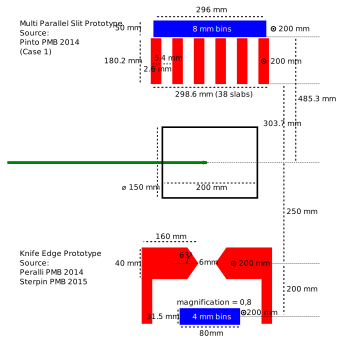
\includegraphics[width=\textwidth]{./figures/detectors_cyl}			
						\caption{\hl{Change the target diameter: 15 cm}}
						\label{CamerasScheme}
					\end{figure}					
				\end{column}				

			\end{columns}

	  \end{block}		
		
		\begin{block}{Results}
			{\Red{\large{AMV}}}
			\begin{table}[h]
			\centering
			\begin{tabular}{llllll}
				\midrule
							& \multicolumn{2}{c}{MPS}												&& \multicolumn{2}{c}{KES}										\\
				\cline{2-3}\cline{5-6}
							& AM 											& MC 									&& AM 										& MC								\\
				\midrule

				Res		& 14.52 mm								& 17.9 mm 	 					&& 13.5 mm								& 13.8 mm						\\
				Eff		& $6.66 \cdot 10^{-4}$  & \tcr{TODO}	&&	$1.06 \cdot 10^{-3}$   & \tcr{TODO}	\\
				\midrule
			\end{tabular}
			\end{table}			
			{\Red{\large{PG profiles detected by the prototypes}}}
% 			\begin{columns}[t]
% 
% 				\begin{column}{0.49\textwidth}			
% 					\includegraphics[width=\textwidth]{./figures/PMMA_phantom-ipnl-auger-notof-1}
% 				
% 				\end{column}			
% 
% 				\begin{column}{0.49\textwidth}
% % 					\begin{figure}
% 						\includegraphics[width=\textwidth]{./figures/PMMA_phantom-iba-auger-notof-3}			
% % 						\caption{\hl{Change the target diameter: 15 cm}}
% % 						\label{CamerasScheme}
% % 					\end{figure}					
% 				\end{column}				

% 			\end{columns}
			
				\begin{figure}
					\includegraphics[width=\textwidth]{./figures/output-crop}			
					\caption{PG profiles: MPS (left), KES (right). See Table~\ref{CamerasParameters} for the parameters.}
					\label{PGprofiles}
				\end{figure}					
				
				
			{\Red{\large{Fall-off Retrieval Precision}}}
			\begin{table}[h]
			\centering
			\begin{tabular}{llllllllllll}
				\midrule
				Time selection 		& \mc{5}{c}{ToF} &   &  \mc{5}{c}{None}     \\
				\cline{2-6}\cline{8-12}
				Energy selection (MeV) 	& \mc{2}{c}{$>1$}    & & \mc{2}{c}{3--6}   & &  \mc{2}{c}{$>1$}    & & \mc{2}{c}{3--6}    \\
				\cline{2-3}\cline{5-6}\cline{8-9}\cline{11-12}
				Camera 						& MPS & KES && MPS & KES & & MPS & KES && MPS & KES \\
				\midrule
				$10^9$ (\# protons)& \textbf{0.37} & 0.55 && 0.44 & 1.07 && 0.42 & 0.74 && 0.66 & \textbf{1.32} \\
				$10^8$    				& \textbf{1.35} & 2.08 && 1.60 & 4.22 && 1.36 & 1.82 && 2.00 & \textbf{9.70} \\
				$10^7$    				& \textbf{4.41} & 11.88 && 20.36 & 20.50 && 22.45 & 17.18 && 56.92 & \textbf{19.39} \\
				\midrule
			\end{tabular}
			\caption{\tcr{TO VERIFY: Standard deviation of the FOP distribution}. In bold, the cuts and ToF selections as proposed.}
			\label{FRPCOMP}
			\end{table}				
		\end{block}

		
		
		
		

	  
	  \vfill
	  
	\end{column}
	
      \end{columns}

      \vfill
%       \vspace{3ex}

	\begin{block}{Acknowledgments}
		\includegraphics[height=0.025\textheight]{./figures/logo_IPNL}
		\hspace{0.025\textwidth}
		\includegraphics[height=0.025\textheight]{./figures/logo-creatis}
		\hspace{0.025\textwidth}		
		
\includegraphics[height=0.025\textheight]{./figures/Logo_LPSC}
		\hspace{0.025\textwidth}
		\includegraphics[height=0.025\textheight]{./figures/logo_primes}
		This work is supported by the Labex PRIMES ANR-11-LABX-0063.
% 		\vspace{2ex}
% 
% 		\begin{center}
% 			\includegraphics[height=0.03\textheight]{./figures/logo_IPNL}
% 			\hspace{0.035\textwidth}
% 			\includegraphics[height=0.03\textheight]{./figures/logo_cnrs_in2p3}
% 			\hspace{0.035\textwidth}
% 			\includegraphics[height=0.03\textheight]{./figures/logo_uni_lyon2}
% 			\hspace{0.035\textwidth}
% 			\includegraphics[height=0.03\textheight]{./figures/logo-creatis}
% 			\hspace{0.035\textwidth}		
% 			\includegraphics[height=0.03\textheight]{./figures/INSA}
% 			\hspace{0.035\textwidth}				
% 			\includegraphics[height=0.03\textheight]{./figures/logo_MI2B}
% 			\hspace{0.035\textwidth}
% 			\includegraphics[height=0.03\textheight]{./figures/logo_primes}
% 		\end{center}
	\end{block}
	
      
    \end{frame}
  \end{document}
